\chapter{Contenido multimedia y streaming}\label{chap:5}
\subsection{Ejercicio 1}
Una vez creado el \Verb#index.html#, se lanza la imagen de docker mediante el
siguiente comando:
\begin{lstlisting}
	docker run --rm -d --network pruebas --name nginx -p 80:80 -v $(pwd)/html/video5/:/usr/share/nginx/html nginx
\end{lstlisting}

Al acceder a \Verb#localhost:80#, se accede correctamente a la página web: \\
\begin{minipage}{\linewidth}
	\centering
	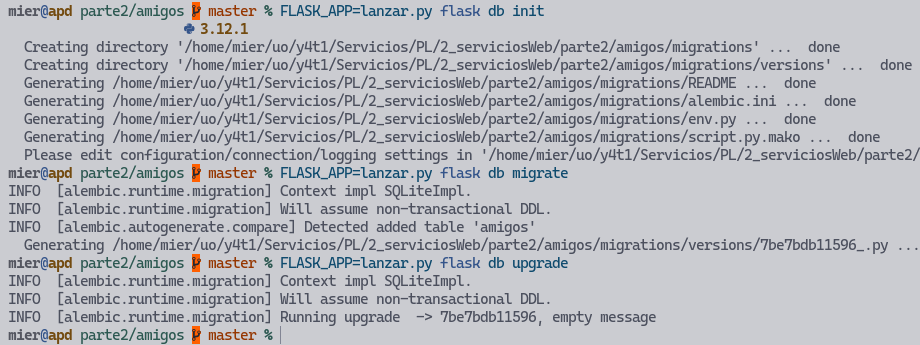
\includegraphics[width=0.8\textwidth]{5/1.png}
	\captionof{figure}{Página web con el vídeo}\label{fig:5/1}
\end{minipage}

Mediante las herramientas de desarrollador, se aprecia que se descargan fragmentos del vídeo
según se necesiten, incluyendo las cabeceras que especifican el rango de bytes a descargar: \\
\begin{minipage}{\linewidth}
	\centering
	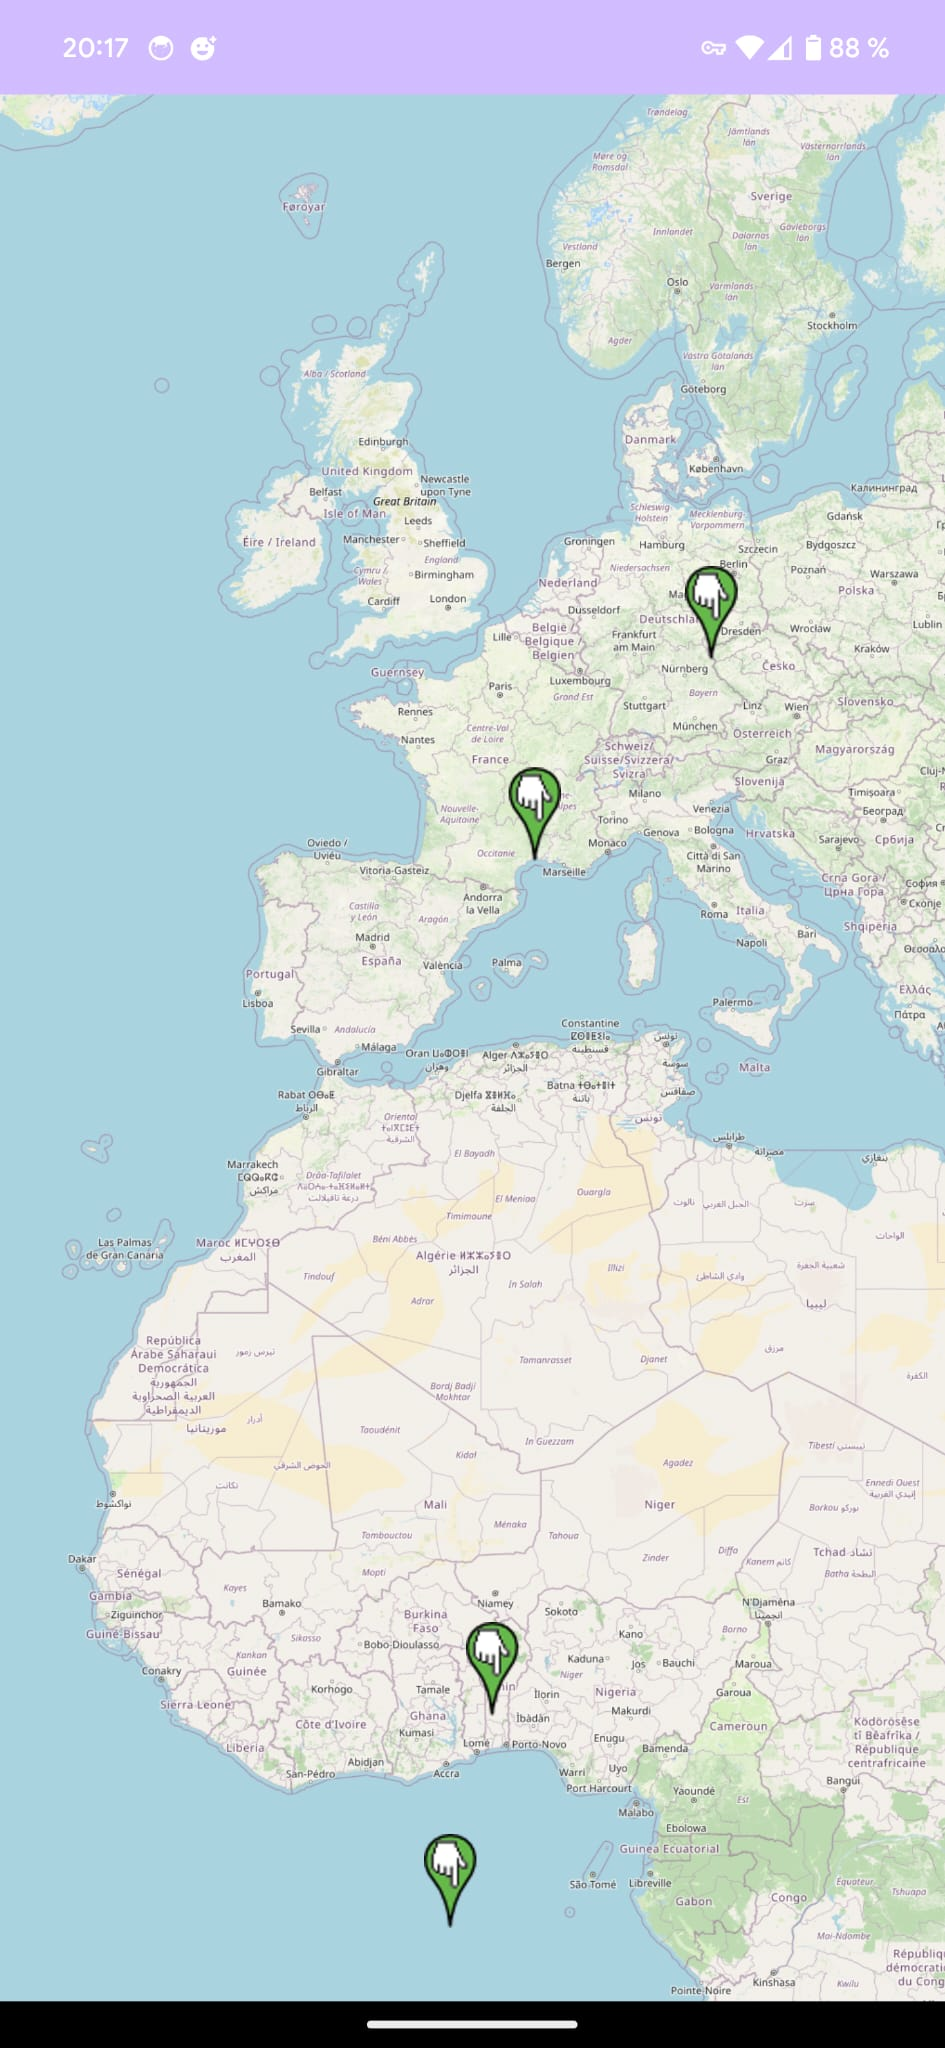
\includegraphics[width=0.8\textwidth]{5/2.png}
	\captionof{figure}{Cabeceras de la descarga del vídeo}\label{fig:5/2}
\end{minipage}

\textbf{Modifica ahora la página y utiliza como fuente otro vídeo} \\
En mi caso, Firefox en Linux admite los tres formatos disponibles (\Verb#mp4#, \Verb#webm# y \Verb#ogv#).
|TODO| revisar

\textbf{Modifica la página anterior para incluir todas las fuentes disponibles}
\begin{lstlisting}[language=html]
	<html lang="es">
	<body>
		<h1><a href="https://mier.info">Prueba de contenido multimedia</a></h1>
		<video width="640" height="360" controls>
			<source src="big_buck_bunny.ogv"  type="video/ogg; codecs=theora">
			<source src="big_buck_bunny.mp4"  type="video/mp4; codecs=avc1.42E01E,mp4a.40.2">
			<source src="big_buck_bunny.webm" type="video/webm; codecs=vp8,vorbis">

			<object type="application/x-shockwave-flash"
					data="http://releases.flowplayer.org/swf/flowplayer-3.2.1.swf"
					width="640" height="360">
				<param name="flashvars"
						value='config={"clip":"http://host/ruta/big_buck_bunny.mp4"}'/>
				<!-- Fallback final: -->
				<p>No se puede reproducir el video</p>
			</object>
		</video>
	</body>
	</html>
\end{lstlisting}
\newpage{} % holi :)
\subsection{Ejercicio 2.~videojs}
\begin{lstlisting}[language=html]
	<html>
	<head>
		<link href="https://vjs.zencdn.net/8.6.1/video-js.css" rel="stylesheet" />
	</head>

	<body>
		<video
			id="my-video"
			class="video-js"
			controls
			preload="auto"
			width="640"
			height="264"
			poster="MY_VIDEO_POSTER.jpg"
			data-setup="{}"
		>
			<source src="big_buck_bunny.mp4" type="video/mp4" />
			<source src="big_buck_bunny.webm" type="video/webm" />
			<p class="vjs-no-js">
			To view this video please enable JavaScript, and consider upgrading to a
			web browser that
			<a href="https://videojs.com/html5-video-support/" target="_blank">supports HTML5 video</a>
			</p>
		</video>

		<script src="https://vjs.zencdn.net/8.6.1/video.min.js"></script>
	</body>
	</html>
\end{lstlisting}
